% 4 · Results. One \subsection per objective; each gets a light divider.
% Frame titles are the EXPECTED claims from the plan. Rewrite them as the actual findings.
\section{Results}

% ================================================================ O1
\subsection{O1 · Energy and carbon}

\begin{frame}{US data-centre electricity growth rose from 7\% to 18\% a year}
  \centering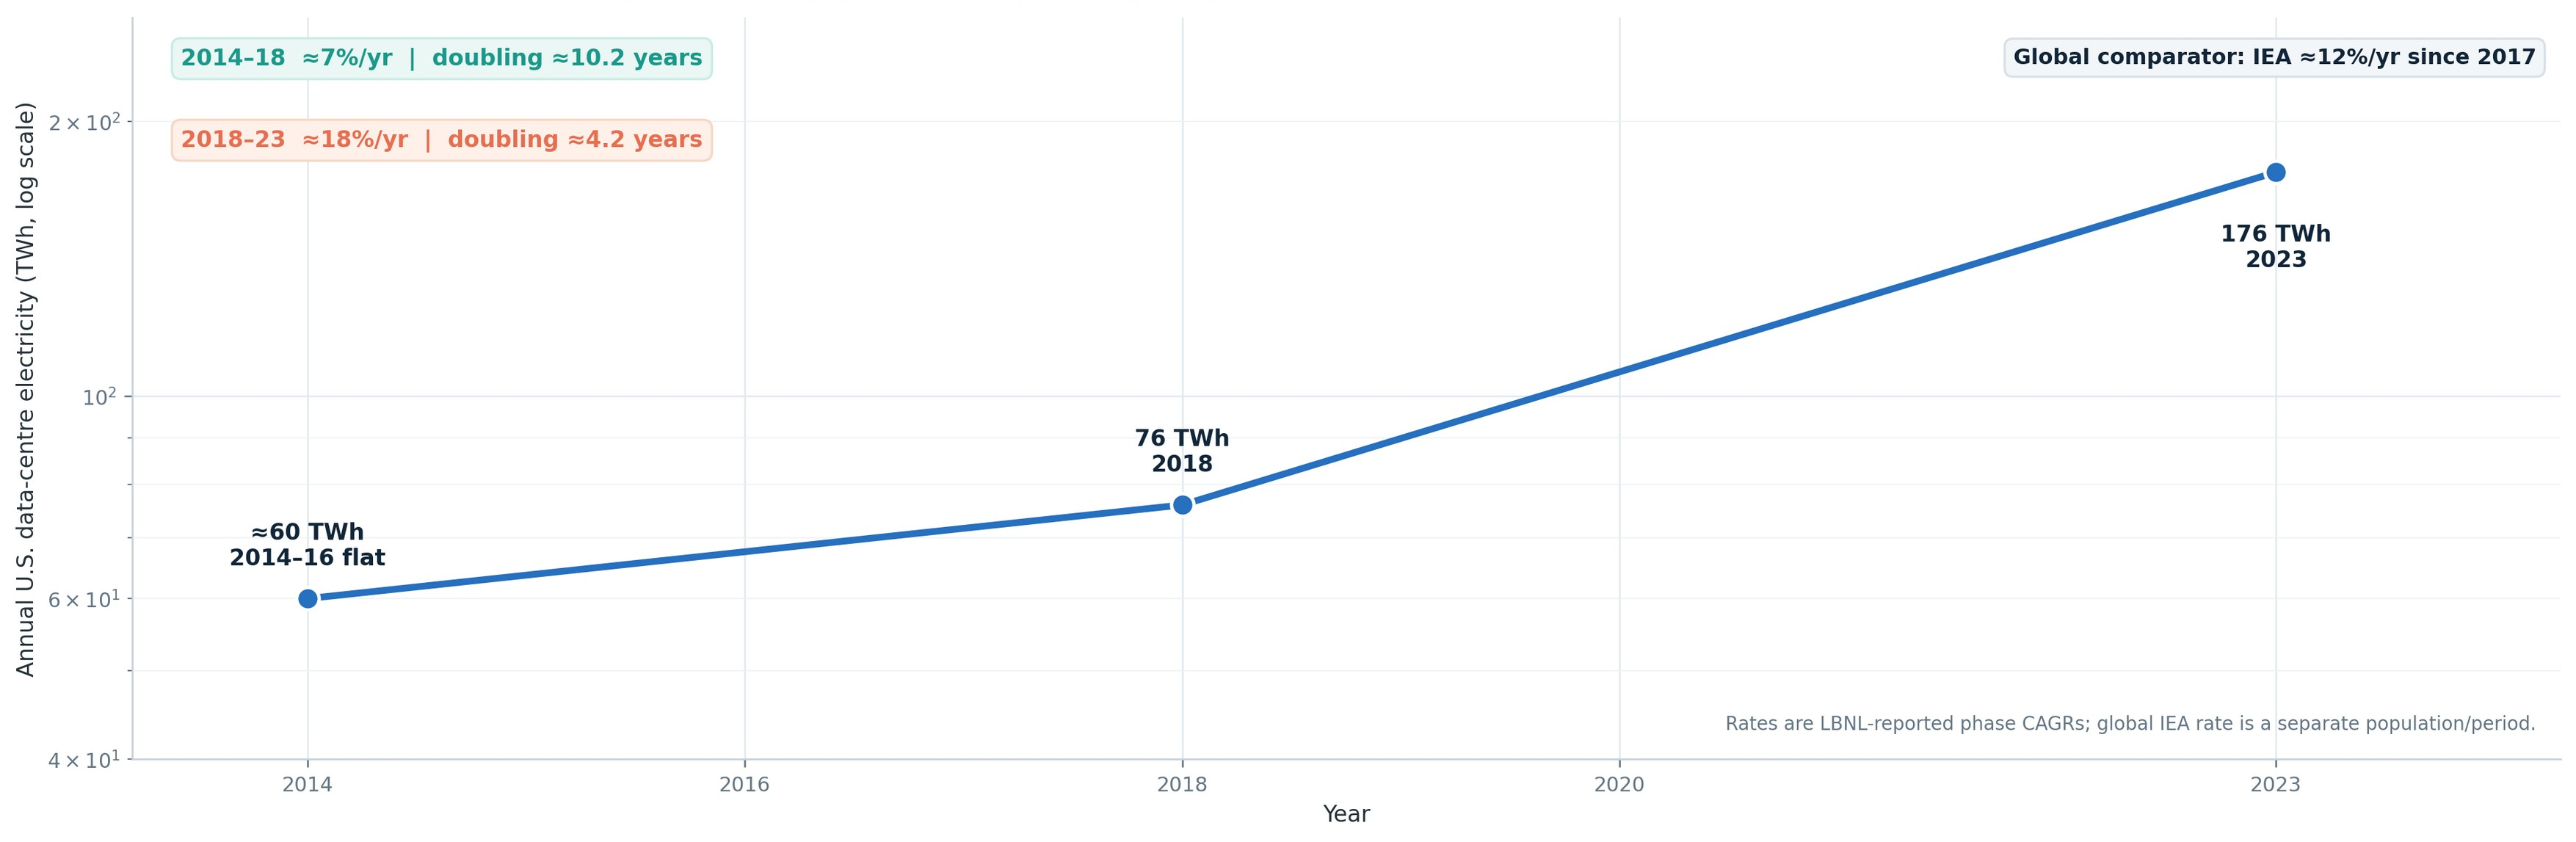
\includegraphics[width=.88\textwidth]{pics/aditya/electricity_growth_crop.png}\par\smallskip
  \raggedright
  \begin{columns}[T,onlytextwidth]
    \column{.56\textwidth}
    {\scriptsize\renewcommand{\arraystretch}{1.25}
    \begin{tabular}{@{}lrr@{}}
      \toprule
      Phase (US, LBNL) & r (\%/yr) & $T_2$ (yr) \\
      \midrule
      \textcolor{phaseCloud}{Cloud, 2014–18 ($\approx$60 → 76 TWh)} & $\approx$7 & $\approx$10.2 \\
      \textcolor{phaseAI}{AI, 2018–23 (76 → 176 TWh)} & $\approx$18 & $\approx$4.2 \\
      \bottomrule
    \end{tabular}\par}
    \column{.4\textwidth}
    {\scriptsize The doubling time fell from about 10 to about 4 years. Globally the IEA estimates
    $\approx$12\%/yr since 2017: a separate series, not spliced in.\par}
  \end{columns}
  \src{Shehabi et al.\ (2024) LBNL-2001637 (growth rates as stated in its executive summary); IEA (2025) \emph{Energy and AI}}
  \note{%
    \NoteKey{US data-centre electricity growth jumped from about 7\% a year to about 18\% a year.}
    \NoteSlide{A line on a log scale, so a steeper line means faster growth: $\approx$60 TWh in 2014--16, 76 TWh in 2018,
    176 TWh in 2023 (Lawrence Berkeley National Lab). The table: cloud era $\approx$7\%/yr, doubling every $\approx$10
    years; AI era $\approx$18\%/yr, doubling every $\approx$4 years.}
    \NoteWhy{The first hard evidence that the AI era breaks the cloud-era plateau.}
    \NoteSay{40}{Here is US data-centre electricity from Lawrence Berkeley National Lab. From 2014 to 2018 it grew about 7\%
    a year, doubling roughly every ten years. From 2018 to 2023 it grew 18\% a year, doubling every four years. That is
    the AI build-out showing up in the electricity data.}
    \begin{NoteAsk}
      \item \emph{And globally?} The IEA estimates about 12\% a year since 2017. That is a different series, so we do not
        splice it in.
    \end{NoteAsk}
  }
\end{frame}

\begin{frame}{One growth table for the three phases}{}
  {\scriptsize\renewcommand{\arraystretch}{1.04}
  \begin{tabularx}{\textwidth}{@{}l X l r r l l@{}}
    \toprule
    Phase & Series & Period & r (\%/yr) & $T_2$ (yr) & 95\% CI & Basis \\
    \midrule
    \textcolor{phaseGA}{\textbf{Great Accel.}} & World primary energy & 1950–2010 & 2.4 & 30 & 28–32 & 48 years \\
    \textcolor{phaseCloud}{\textbf{Cloud era}} & World primary energy & 2010–19 & 1.2 & 58 & 51–66 & 10 years \\
     & Data-centre electricity, world & 2010–18 & 0.7 & $\approx$95 & – & 2 values \\
     & Data-centre electricity, US & 2014–18 & $\approx$7 & $\approx$10 & – & LBNL \\
    \textcolor{phaseAI}{\textbf{AI era}} & Data-centre electricity, US & 2018–23 & $\approx$18 & $\approx$4.2 & – & LBNL \\
     & Data-centre electricity, world & 2024–30 & 14.7 & 5.1 & – & IEA proj. \\
     & AI training compute & 2010–26 & 329 & 0.48 & 0.45–0.51 & 478 models \\
    \bottomrule
  \end{tabularx}}
  \par\smallskip
  {\scriptsize\textbf{Breakpoint test} (two-segment fit): AI compute breaks in \textbf{2011} (doubling 1.7 → 0.5 years).
  World energy: 1974 over 1950–2019, but window-dependent (2011 over 1990–2019); 1950 cannot be tested, as data before
  1965 are decadal. Data-centre electricity: too few points.\par}
  \begin{block}{Our comment}\scriptsize
    Compute took off in 2011, yet data-centre electricity rose only 6\% in 2010–18. PUE stopped improving around 2014;
    the 2018 jump matches AI-server demand (<2 → >40 TWh). Chip efficiency not tested.
  \end{block}
  \src{Our World in Data; Masanet et al.\ (2020); Shehabi et al.\ (2024); IEA (2025); Epoch AI. analysis/growth\_table.py}
  \note{%
    \NoteKey{On one scale, the cloud era is the flat exception, and AI compute is the fastest thing in the table.}
    \NoteSlide{Each row: annual growth $r$, doubling time $T_2$, and a 95\% interval where yearly data exist. World energy
    doubled every 30 years (1950--2010); world data-centre electricity barely moved (2010--18); US data-centre electricity
    doubles every 4 years (2018--23); AI training compute doubles every 6 months.}
    \NoteSay{50}{This puts all three phases on one scale. In the Great Acceleration, world energy doubled about every 30
    years. In the cloud era, data-centre electricity barely moved: plus 6\% in eight years. In the AI era, US
    data-centre electricity doubles every four years. The driver is the bottom row: AI training compute doubles every
    six months. Compute jumped in 2011, yet electricity only turned up around 2018. Building efficiency stopped
    improving around 2014, so the 2018 jump lines up with the arrival of AI servers rather than with PUE.}
    \begin{NoteAsk}
      \item \emph{No intervals for data-centre electricity?} Only a few published points exist; an interval needs a
        yearly series.
      \item \emph{Do the phases start in 1950 and 2010?} Compute breaks in 2011. For world energy it depends on the
        window (1974 over 1950--2019; 2011 over 1990--2019), and 1950 itself cannot be tested.
    \end{NoteAsk}
  }
\end{frame}

\begin{frame}{AI servers' electricity grew more than 20-fold while facility efficiency stalled}
  \centering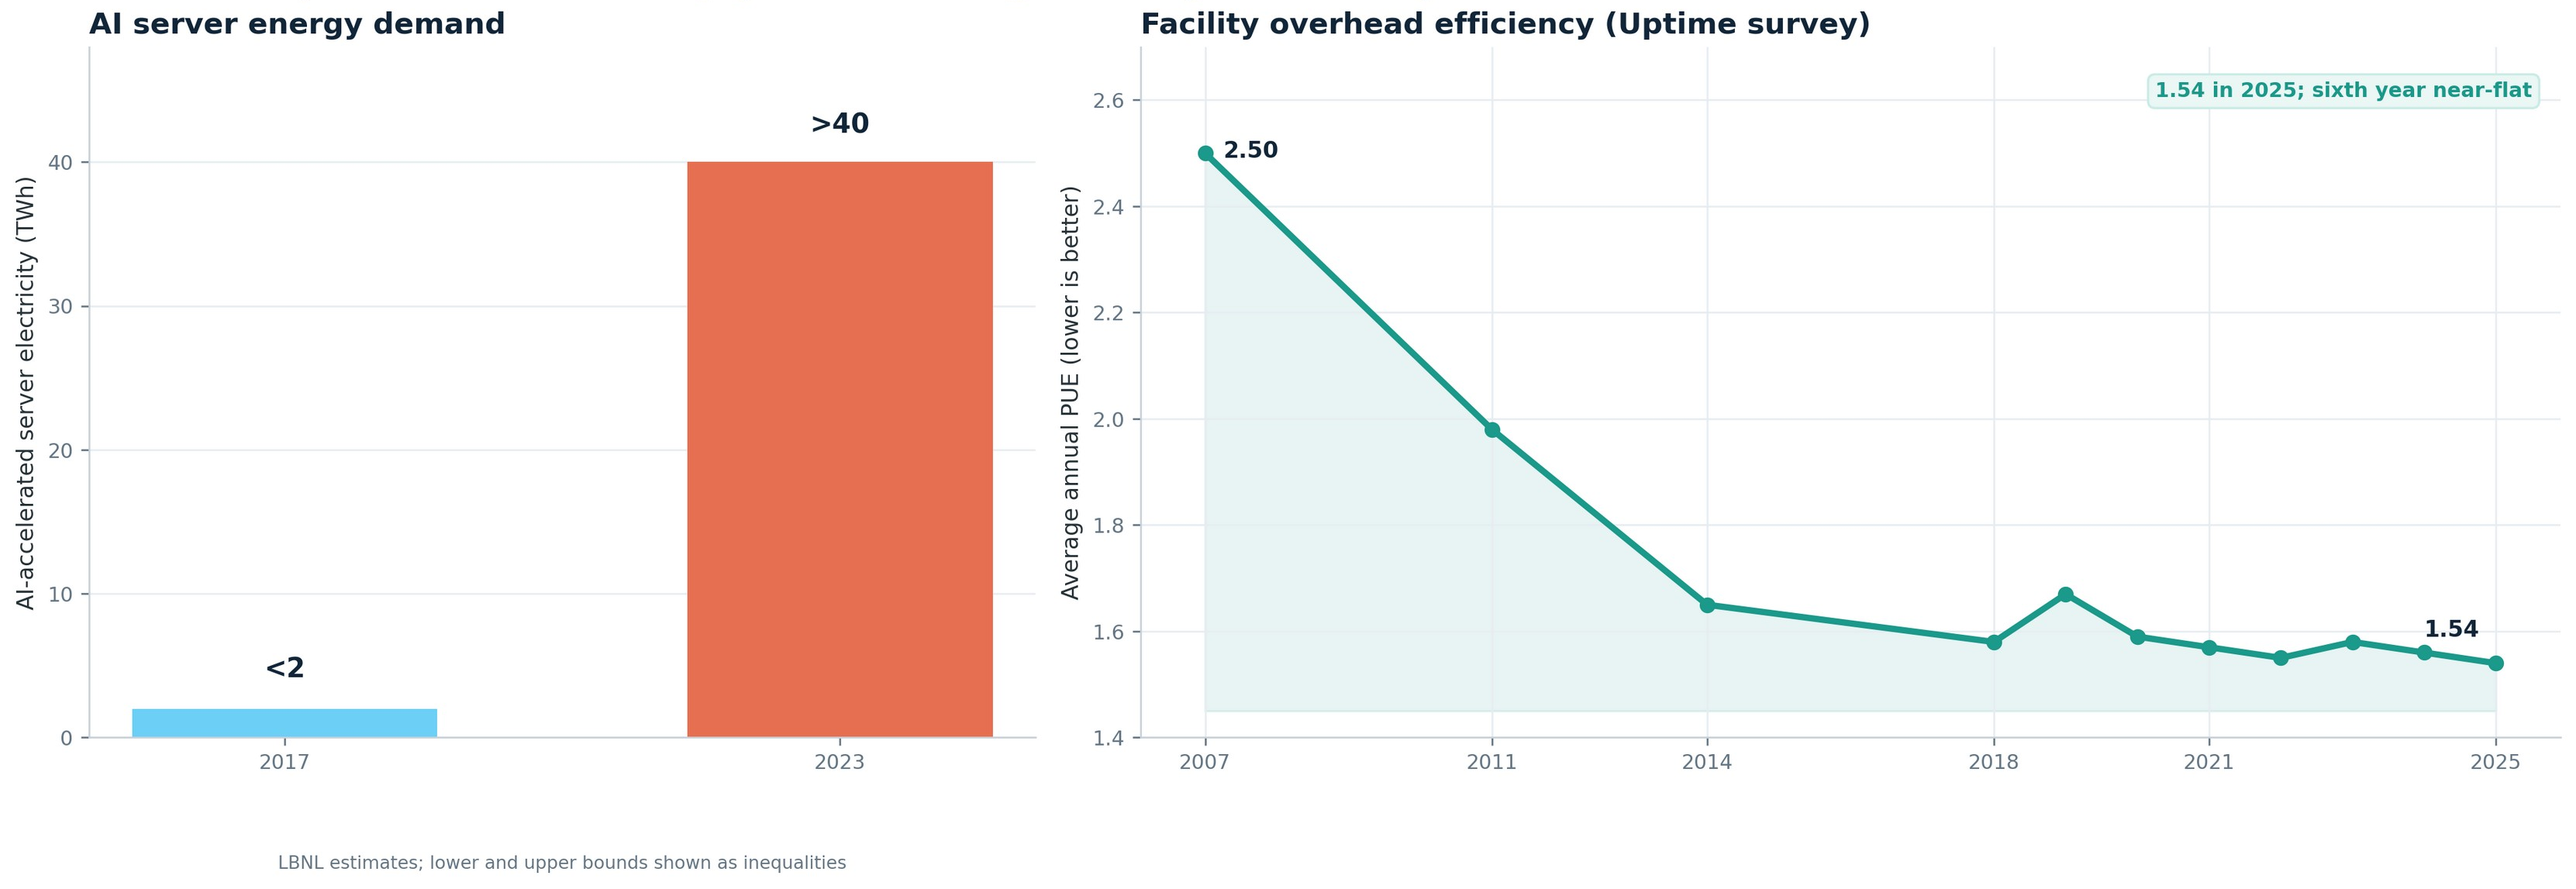
\includegraphics[width=.94\textwidth]{pics/aditya/compute_efficiency_crop.png}\par\smallskip
  \raggedright
  \begin{itemize}\footnotesize
    \item US AI-accelerated servers: under 2 TWh in 2017, over 40 TWh in 2023
    \item Average PUE fell from 2.50 (2007) to 1.65 (2014), then stayed near 1.5 (1.54 in 2025): the easy gains are used up
    \item PUE measures facility overhead, not chip efficiency: we did not test performance per watt
  \end{itemize}
  \src{Shehabi et al.\ (2024) LBNL; Uptime Institute (2025) \emph{Global Data Center Survey}}
  \note{%
    \NoteKey{AI servers' electricity rose more than 20-fold while the easy efficiency gains ran out.}
    \NoteSlide{Left: US AI-accelerated servers used under 2 TWh in 2017 and over 40 TWh in 2023. Right: the average PUE of
    data centres fell from 2.50 (2007) to 1.65 (2014), then stayed around 1.5--1.6 (1.54 in 2025).}
    \NoteWhy{In the cloud era, better buildings (lower PUE) offset growth. That lever is mostly used up, so growth in
    computing now shows up as growth in electricity.}
    \NoteSay{40}{Why did the plateau end? On the left, electricity used by AI servers in the US went from under 2 to over 40
    terawatt-hours in six years. On the right, the efficiency of the buildings: PUE fell fast until 2014 and has been
    almost flat for years. The one-off gains, like better cooling and moving to big efficient sites, are used up.}
    \begin{NoteAsk}
      \item \emph{But chips keep getting more efficient?} Yes. PUE measures the building, not the chip; we did not test
        chip efficiency.
    \end{NoteAsk}
  }
\end{frame}

\begin{frame}{The load sits in three regions; its carbon depends on each grid}
  \centering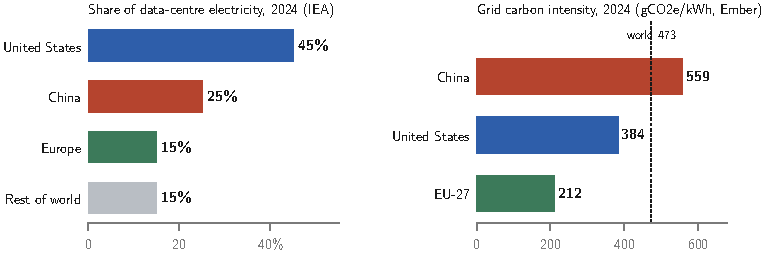
\includegraphics[width=\textwidth]{figs/o1_regional_carbon.pdf}\par\smallskip
  \raggedright
  \begin{itemize}\footnotesize
    \item The same kWh emits about 2.6 times as much CO\textsubscript{2} in China (559 g) as in the EU (212 g)
    \item Electricity is a regional load; carbon is a global impact, set by the local grid mix
    \item The EU-27 is a proxy for the IEA's ``Europe''; intensities are benchmarks, not emission estimates
  \end{itemize}
  \src{IEA (2025) \emph{Energy and AI}; Ember (2026) yearly electricity data, 2024 values (analysis/o1\_regional.py)}
  \note{%
    \NoteKey{Where the electricity is used decides how much CO\textsubscript{2} it emits.}
    \NoteSlide{Left: share of data-centre electricity in 2024: US 45\%, China 25\%, Europe 15\%, rest 15\% (IEA). Right: grid
    carbon intensity in 2024, grams of CO\textsubscript{2} per kWh: China 559, US 384, EU 212; dashed line = world 473
    (Ember).}
    \NoteWhy{The same kWh emits about 2.6 times more CO\textsubscript{2} in China than in the EU. Electricity is a regional
    load; carbon is a global impact.}
    \NoteSay{35}{Electricity use sits in three regions. But what it emits depends on each grid: a kilowatt-hour in China
    emits about two and a half times as much CO\textsubscript{2} as one in the EU. So the electricity is a regional
    problem, for grids and local air, while the carbon adds to a global one.}
    \begin{NoteAsk}
      \item \emph{Are these data-centre emissions?} No: they are grid averages, used as benchmarks. The EU stands in for
        the IEA's ``Europe''.
    \end{NoteAsk}
  }
\end{frame}

% ================================================================ O2
\subsection{O2 · Materials, water and waste}

\begin{frame}{The AI build-out is heading into dry basins}
  \centering
  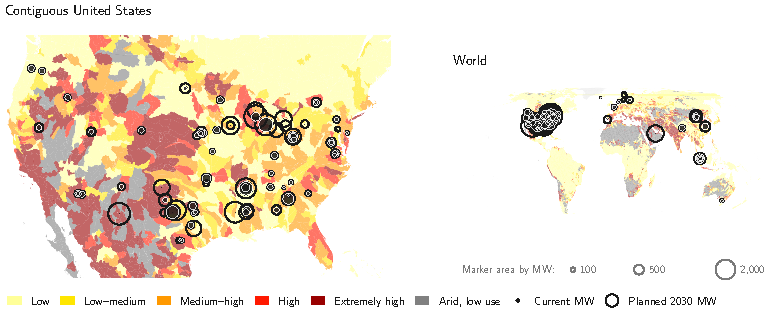
\includegraphics[width=\textwidth]{figs/o2a_sites_water_stress.pdf}\par
  \raggedright\scriptsize 96 AI data centres: 15 GW today, 50 GW planned by 2030. Many of the largest
  planned sites, in West Texas, New Mexico, Abu Dhabi and Inner Mongolia, sit in high or extremely high stress.
  \src{Epoch AI (2026), geocoded via OpenStreetMap; WRI Aqueduct 4.0 baseline water stress}
  \note{%
    \NoteKey{Much of the planned AI build-out is heading into water-stressed river basins.}
    \NoteSlide{Background colour = Aqueduct water stress (yellow = low, dark red = extremely high, grey = arid with little
    use). Filled dot = a site's power today; open ring = planned by 2030. 96 sites: 15 GW today, 50 GW planned.}
    \NoteSay{50}{I worked on water, materials and waste. We took Epoch AI's 96 AI data centres, about 15 gigawatts today and
    50 planned by 2030, and placed each on WRI's water-stress map. Two things stand out. The rings are much bigger than
    the dots: most of this capacity is not built yet. And many of the biggest rings sit in red: Stargate in New Mexico,
    Shackelford and the Texas Panhandle, Stargate UAE in Abu Dhabi, Ulanqab in Inner Mongolia. Not all of them: the
    largest planned site, in Wisconsin, is not stressed. The next slide puts a number on it.}
    \begin{NoteAsk}
      \item \emph{How accurate are the locations?} All 96 were checked against country and state; city-level accuracy is
        enough because basins are tens to hundreds of km across.
      \item \emph{Where is Vizag?} Not in Epoch's data yet; it is case study 2.
    \end{NoteAsk}
  }
\end{frame}

\begin{frame}{By size, 34\% of AI capacity is in stressed basins today, 39–45\% by 2030}
  \begin{columns}[T,onlytextwidth]
    \column{.56\textwidth}
    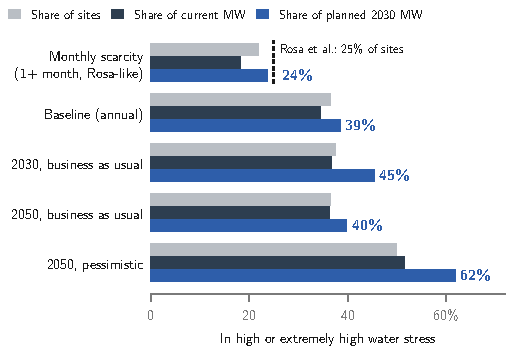
\includegraphics[width=\linewidth]{figs/o2b_count_vs_size.pdf}
    \column{.41\textwidth}
    \begin{itemize}\footnotesize
      \item Today: 37\% of sites, 34\% of MW in high or extremely high stress
      \item Planned MW grows \textbf{3.7×} in stressed basins (3.1× elsewhere): 39\% at today's stress
      \item 45\% at 2030 stress, but most of that step is two Gulf Coast sites near the 40\% line; \textbf{62\%} by 2050, pessimistic
      \item \textbf{21 M} people within 25 km of a stressed site, planned sites included (48 M within 50 km)
      \item Check: our monthly test gives 22\% of sites; Rosa et al.\ 25\%
    \end{itemize}
  \end{columns}
  \src{Epoch AI (2026); WRI Aqueduct 4.0; GHSL GHS-POP 2025; Rosa et al.\ (2026). Annual stress counts all withdrawals, incl.\ power-plant cooling.}
  \note{%
    \NoteKey{Weighted by power, 34\% of AI capacity is in high-stress basins today, 39--45\% by 2030.}
    \NoteSlide{Bars per scenario: grey = share of sites, dark = share of today's MW, blue = share of planned 2030 MW. The
    dashed line is Rosa et al.'s 25\% (a share of sites).}
    \NoteSay{60}{Counting sites treats a 10-megawatt site like a 2-gigawatt campus, so we weight by power. Today, 34\% of AI
    power sits in high-stress basins. Keep today's stress map and look at where new capacity is going: 39\%, because
    capacity in stressed basins grows 3.7 times, against 3.1 elsewhere. With WRI's 2030 projection it is 45\%, but most
    of that step is two big sites in Louisiana and Mississippi sitting just under the 40\% line. In the pessimistic 2050
    case it is 62\%. About 21 million people live within 25 km of a stressed site. As a check, our monthly test gives
    22\% of sites, close to Rosa's 25\%.}
    \begin{NoteAsk}
      \item \emph{Why is 2050 lower than 2030?} The same two Gulf Coast basins fall back below 40\%: a threshold effect.
      \item \emph{Why is Indiana ``high''?} Aqueduct counts all withdrawals, including power-plant cooling water.
    \end{NoteAsk}
  }
\end{frame}

\begin{frame}{Most of the water is used at power plants, not on site}
  \begin{columns}[T,onlytextwidth]
    \column{.56\textwidth}
    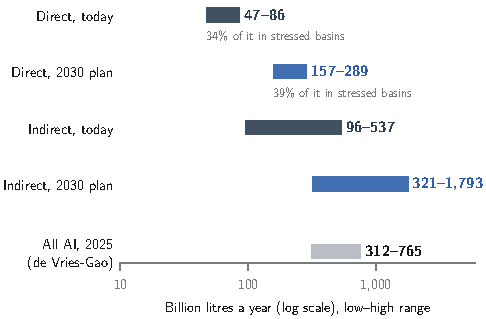
\includegraphics[width=\linewidth]{figs/o2c_water_use.pdf}
    \column{.41\textwidth}
    \begin{itemize}\footnotesize
      \item Today's 15 GW: \textbf{143–624 bn L} a year; the 2030 plan: 478–2,082 bn L
      \item \textbf{67–86\%} of it is indirect, consumed by the power plants
      \item On-site cooling water in stressed basins: 16–30 bn L today, 61–111 bn L by 2030
      \item Reported sites range from 0.001 to 7 L/kWh: cooling design matters more than size
    \end{itemize}
  \end{columns}
  \src{Parameters from de Vries-Gao (2026) \emph{Patterns}: WUE 0.56–1.04 L/kWh, PUE 1.10–1.43, grid 1.04–4.52 L/kWh. Load factor 70–90\% (our assumption). Epoch AI (2026).}
  \note{%
    \NoteKey{Most of the water AI uses is evaporated at power plants, not at the data centre.}
    \NoteSlide{Each bar is a low--high range in billions of litres a year, on a log scale (each gridline is 10$\times$).
    Direct = on-site cooling; indirect = power plants; today and the 2030 plan. Grey = de Vries-Gao's estimate for all
    AI worldwide in 2025. For scale: 1 billion litres $\approx$ 400 Olympic pools.}
    \NoteSay{50}{How much water is that? Today's 15 gigawatts use 143 to 624 billion litres a year; the 2030 plan, 478
    billion to about 2 trillion. The main point: two-thirds to 86\% of that is not at the data centre at all. It
    evaporates at the power plants that feed it. And sites that report water vary by a factor of thousands, from almost
    zero to 7 litres per kWh, so cooling design matters more than size. Our one assumption: sites run at 70 to 90\% of
    their power.}
    \begin{NoteAsk}
      \item \emph{Why such a wide range?} The power-plant factor: 1.04 vs 4.52 litres per kWh in the published sources.
      \item \emph{Consumed or withdrawn?} Consumed (evaporated), on both sides.
    \end{NoteAsk}
  }
\end{frame}

\begin{frame}{Two case studies: a desert city in the US, a port city in India}
  \centering
  \begin{minipage}[t]{.6\textwidth}\centering
    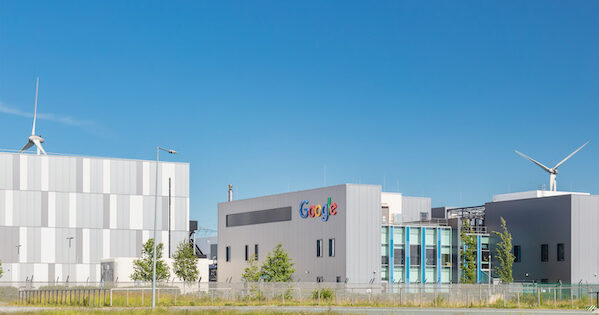
\includegraphics[height=4.3cm]{pics/google_mesa_az.png}\par\smallskip
    {\footnotesize\textbf{Case 1 · Google, Mesa, Arizona}\par}
    {\scriptsize On our map · extremely high water stress\par}
  \end{minipage}\hfill
  \begin{minipage}[t]{.36\textwidth}\centering
    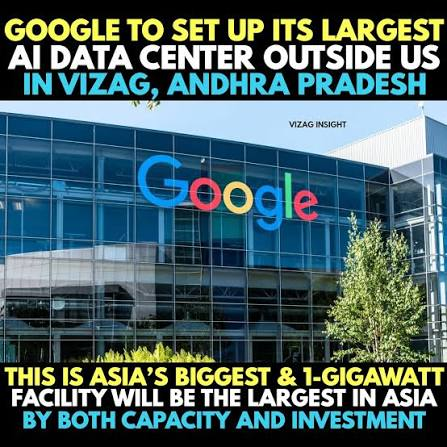
\includegraphics[height=4.3cm]{pics/vishakhapatnam_image.png}\par\smallskip
    {\footnotesize\textbf{Case 2 · Google–AdaniConneX, Visakhapatnam}\par}
    {\scriptsize Planned 1 GW · not yet in the Epoch data\par}
  \end{minipage}
  \src{Left: illustrative photo of a Google data centre, not the Mesa site. Right: announcement as reported on social media (Vizag Insight); the photo is a Google office, not the Vizag site.}
  \note{%
    \NoteKey{Two case studies, chosen to contrast: a US desert city on our map, an Indian port city not yet in the data.}
    \NoteSlide{Two pictures. The left one is a Google data centre, but not the Mesa site. The right one is the announcement
    as it circulated on social media.}
    \NoteSay{20}{Totals hide what happens in one place, so we picked two case studies from official records and news reports:
    a desert city in the US that is on our map, and a port city in India that is not in the data yet.}
  }
\end{frame}

\begin{frame}{Case 1 · Google Mesa: a desert site whose water travels \textasciitilde300 km}
  \begin{columns}[T,onlytextwidth]
    \column{.53\textwidth}
    \begin{itemize}\footnotesize
      \item On our map: 183 MW today, 237 MW planned. Its basin is in \textbf{extremely high} stress;
        withdrawals exceed supply in \textbf{all 12 months}
      \item Google's deal with the city (reported 2020): 1 million gallons a day guaranteed, up to 4 million:
        \textbf{15 million L a day}, 5.5 bn L a year
      \item 2021, Mesa's next data centre (Facebook-linked): Vice Mayor Jenn Duff, the only vote against,
        called data centres ``an irresponsible use of our water''
      \item The canal's river is shrinking: in August 2026 the federal government cut Lower Basin
        allocations by 1.25 million acre-feet a year for 2027–28
    \end{itemize}
    \column{.43\textwidth}
    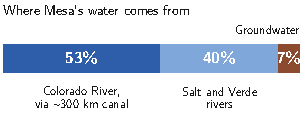
\includegraphics[width=\linewidth]{figs/case_mesa.pdf}\par\smallskip
    \begin{block}{Our comment}\footnotesize
      The stress is local, the source distant: over half of Mesa's water comes by canal from a
      river already being cut.
    \end{block}
  \end{columns}
  \src{City of Mesa water supply page (2026); US Bureau of Reclamation (CAP; news release 21 Aug 2026); Bloomberg (1 Apr 2020); NBC News (19 Jun 2021); Epoch AI; WRI Aqueduct 4.0}
  \note{%
    \NoteKey{A data centre in a desert basin that already uses more water than it gets, fed by a shrinking river 300 km away.}
    \NoteSlide{Facts on the left. The bar shows where Mesa's water comes from: 53\% Colorado River (via the Central Arizona
    Project canal), 40\% Salt and Verde rivers, 7\% groundwater. One acre-foot $\approx$ 1.23 million litres.}
    \NoteSay{60}{Mesa is a suburb of Phoenix. Google's site there is 183 megawatts today, 237 planned. Its basin uses more
    water than it renews in every month of the year. Google's deal with the city, reported in 2020, guarantees a million
    gallons a day and allows up to four million, about 15 million litres. In 2021, when the city approved its next data
    centre, the vice mayor cast the only vote against, calling data centres an irresponsible use of water. More than half
    of Mesa's water is Colorado River water carried about 300 km by canal, and in August 2026 the federal government cut
    Lower Basin allocations by 1.25 million acre-feet a year. The stress is local; the source is distant and shrinking.}
    \begin{NoteAsk}
      \item \emph{Does Google use 4 million gallons a day?} That is the ceiling in the deal; actual use is not disclosed.
    \end{NoteAsk}
  }
\end{frame}

\begin{frame}{Case 2 · Visakhapatnam: a gigawatt AI hub in a city already 15\% short}
  \begin{columns}[T,onlytextwidth]
    \column{.53\textwidth}
    \begin{itemize}\footnotesize
      \item Google with AdaniConneX and Airtel: \textbf{1 GW}, about US\$15 bn; foundation stone laid April 2026 (Tarluvada)
      \item The city receives \textbf{410 of the 480 million L} a day it needs
      \item The environmental clearance does not disclose water use in operation; the state says
        water will come from Polavaram by dedicated pipeline
      \item Google and AdaniConneX say they will air-cool. Residents protest: ``We cannot drink data''
    \end{itemize}
    \column{.43\textwidth}
    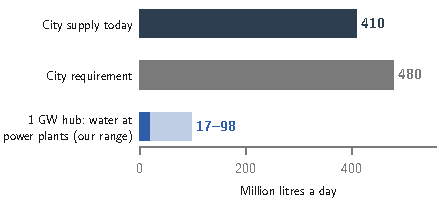
\includegraphics[width=\linewidth]{figs/case_vizag.pdf}\par\smallskip
    \begin{block}{Our comment}\footnotesize
      Our check: medium–high stress basin (20–40\%). Air cooling saves on-site water, but the power
      plants, wherever they are, would still use \textbf{17–98 million L a day}: equal to 4–24\% of the city's supply.
    \end{block}
  \end{columns}
  \src{The Federal (27 Oct 2026); Mongabay India (12 May 2026); Google (Oct 2025). Our estimate uses the slide-24 ranges (US-derived grid water intensity).}
  \note{%
    \NoteKey{A planned 1 GW AI hub in a city that already lacks 15\% of the water it needs.}
    \NoteSlide{Facts on the left. The bar: the city gets 410 million litres a day but needs 480; our estimate for the hub's
    power-plant water is 17--98 million litres a day.}
    \NoteSay{60}{In October 2025 Google announced a 1-gigawatt AI hub in Visakhapatnam with AdaniConneX and Airtel, about 15
    billion dollars. The city already gets only 410 of the 480 million litres a day it needs. The environmental clearance
    does not say how much water the site will use once running; the state says water will come by pipeline from
    Polavaram, about 190 km away; the companies say they will use air cooling. Residents protested: ``We cannot drink
    data.'' Our check: air cooling removes only the on-site water. The power plants, wherever they are, would still evaporate 17 to 98
    million litres a day, equal to 4 to 24\% of what the whole city gets.}
    \begin{NoteAsk}
      \item \emph{Does that come from the city's pipes?} Not necessarily: it compares scale, not the same supply.
      \item \emph{Reports of a 2.51 GW clearance?} Recent press reports it; we use Google's announced 1 GW.
    \end{NoteAsk}
  }
\end{frame}

\begin{frame}{Minerals come from a few countries; e-waste collection is very uneven}
  \centering
  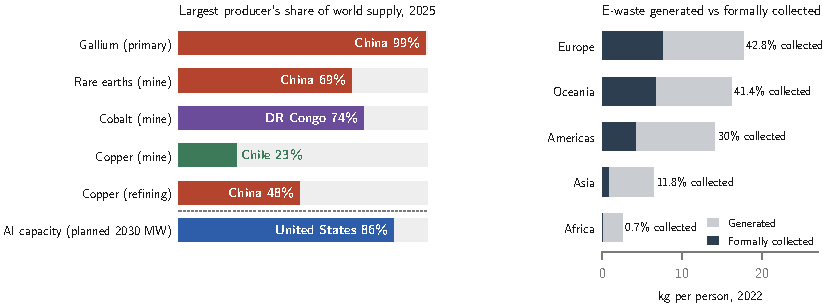
\includegraphics[width=\textwidth]{figs/o2d_materials_ewaste.pdf}\par
  \vspace{4pt}\raggedright\scriptsize Gallium and rare earths come mostly from China and cobalt from DR Congo;
  86\% of planned AI capacity is in the US. China's December 2024 ban on gallium and germanium exports to the
  US is suspended only until 27~Nov~2026. E-waste: 62 Mt in 2022, 22\% formally collected; in Africa, under 1\%.
  \src{USGS Mineral Commodity Summaries 2026; Baldé et al.\ (2024) \emph{Global E-waste Monitor}; Epoch AI (2026)}
  \note{%
    \NoteKey{The minerals come from a few countries, the demand from the US, and e-waste is handled very differently by region.}
    \NoteSlide{Left: the largest producer's share of world supply in 2025 (USGS): China 99\% of gallium (chips, power
    electronics), 69\% of rare earths (magnets), 48\% of refined copper (wiring); DR Congo 74\% of cobalt (batteries).
    Bottom bar: 86\% of planned AI capacity is in the US. Right: e-waste per person in 2022, with the formally collected
    part in dark: Europe 43\%, Africa 0.7\%.}
    \NoteSay{50}{Last, materials and waste. A handful of countries supply the key minerals: China produces almost all
    gallium and most rare earths, DR Congo most cobalt, while the demand sits in the US. And supply can be cut: China's
    ban on gallium and germanium exports to the US is only suspended until 27 November 2026. E-waste ends up in a third
    region: Europe formally collects 43\% of its e-waste, Africa under 1\%. For minerals the impact is displaced, far
    from where the chips are used; for e-waste we can only show that collection is very uneven.}
    \begin{NoteAsk}
      \item \emph{How much of these minerals goes to AI?} The USGS does not break that out; the slide is about
        concentration.
      \item \emph{Does AI e-waste end up in Africa?} We did not trace that: the data cover all electronics.
      \item \emph{Check before presenting:} has the 27 Nov 2026 suspension been extended?
    \end{NoteAsk}
  }
\end{frame}

\begin{frame}{Against a global boundary AI's water barely registers; in a basin it does}
  \small The Earth3 model (Collste et al.\ 2018) tracks freshwater as one global number: withdrawals below
  3,000 km\textsuperscript{3} a year are safe, above 4,000 high-risk.
  \vspace{5pt}

  \centering
  \bignum[phaseAI]{<0.1\%}{of Earth3's safe limit: the 2030 plan uses 0.5–2.1 km\textsuperscript{3} a year}\hfill
  \bignum[phaseAI]{12 of 12}{months a year with withdrawals above supply in Google Mesa's basin}\hfill
  \bignum[phaseAI]{15\% short}{Visakhapatnam gets 410 of the 480 million L a day it needs}
  \vspace{5pt}

  \raggedright
  \begin{block}{Our comment}\footnotesize
    A single global number averages away exactly where the pressure is. AI's water use has to be judged
    basin by basin, and city by city.
  \end{block}
  \src{Collste et al.\ (2018) Earth3 technical notes, p.\,27 (thresholds as in Steffen et al.\ 2015); our estimates, slides 24, 26, 27. Earth3 counts withdrawals; ours is consumption, so withdrawals would be larger.}
  \note{%
    \NoteKey{Against the planet's freshwater limit AI barely registers; in particular basins it does.}
    \NoteSlide{The Earth3 model sets a global freshwater limit: withdrawals under 3,000 km\textsuperscript{3} a year are safe,
    over 4,000 high-risk (1 km\textsuperscript{3} = a trillion litres). Three numbers: $<$0.1\% (the 2030 plan's 0.5--2.1
    km\textsuperscript{3}), 12 of 12 months over supply in Mesa's basin, and Vizag already 15\% short of the water it needs.}
    \NoteWhy{Water cannot move between basins the way CO\textsubscript{2} mixes in the air, so a global total is the wrong
    yardstick for water.}
    \NoteSay{45}{To close my part, back to planetary boundaries. On Earth3's global freshwater scale, the entire 2030 AI plan
    is less than a tenth of a percent: it barely registers. But Mesa's basin already uses more than it gets every month,
    and Visakhapatnam already gets 15\% less water than it needs, before a gigawatt hub arrives. So AI's water has to be
    judged basin by basin. Next: who bears these costs.}
    \begin{NoteAsk}
      \item \emph{So it is not bad globally?} For water, yes, it is small. For carbon, the global total is what counts, and
        it is growing fast (O1).
      \item \emph{Withdrawal vs consumption?} Earth3 counts withdrawals; ours is consumption, so the true share is larger.
    \end{NoteAsk}
  }
\end{frame}

% ================================================================ O3
\subsection{O3 · Economy, politics and society}

\begin{frame}{Tracked AI capacity is far more concentrated than population}
  \centering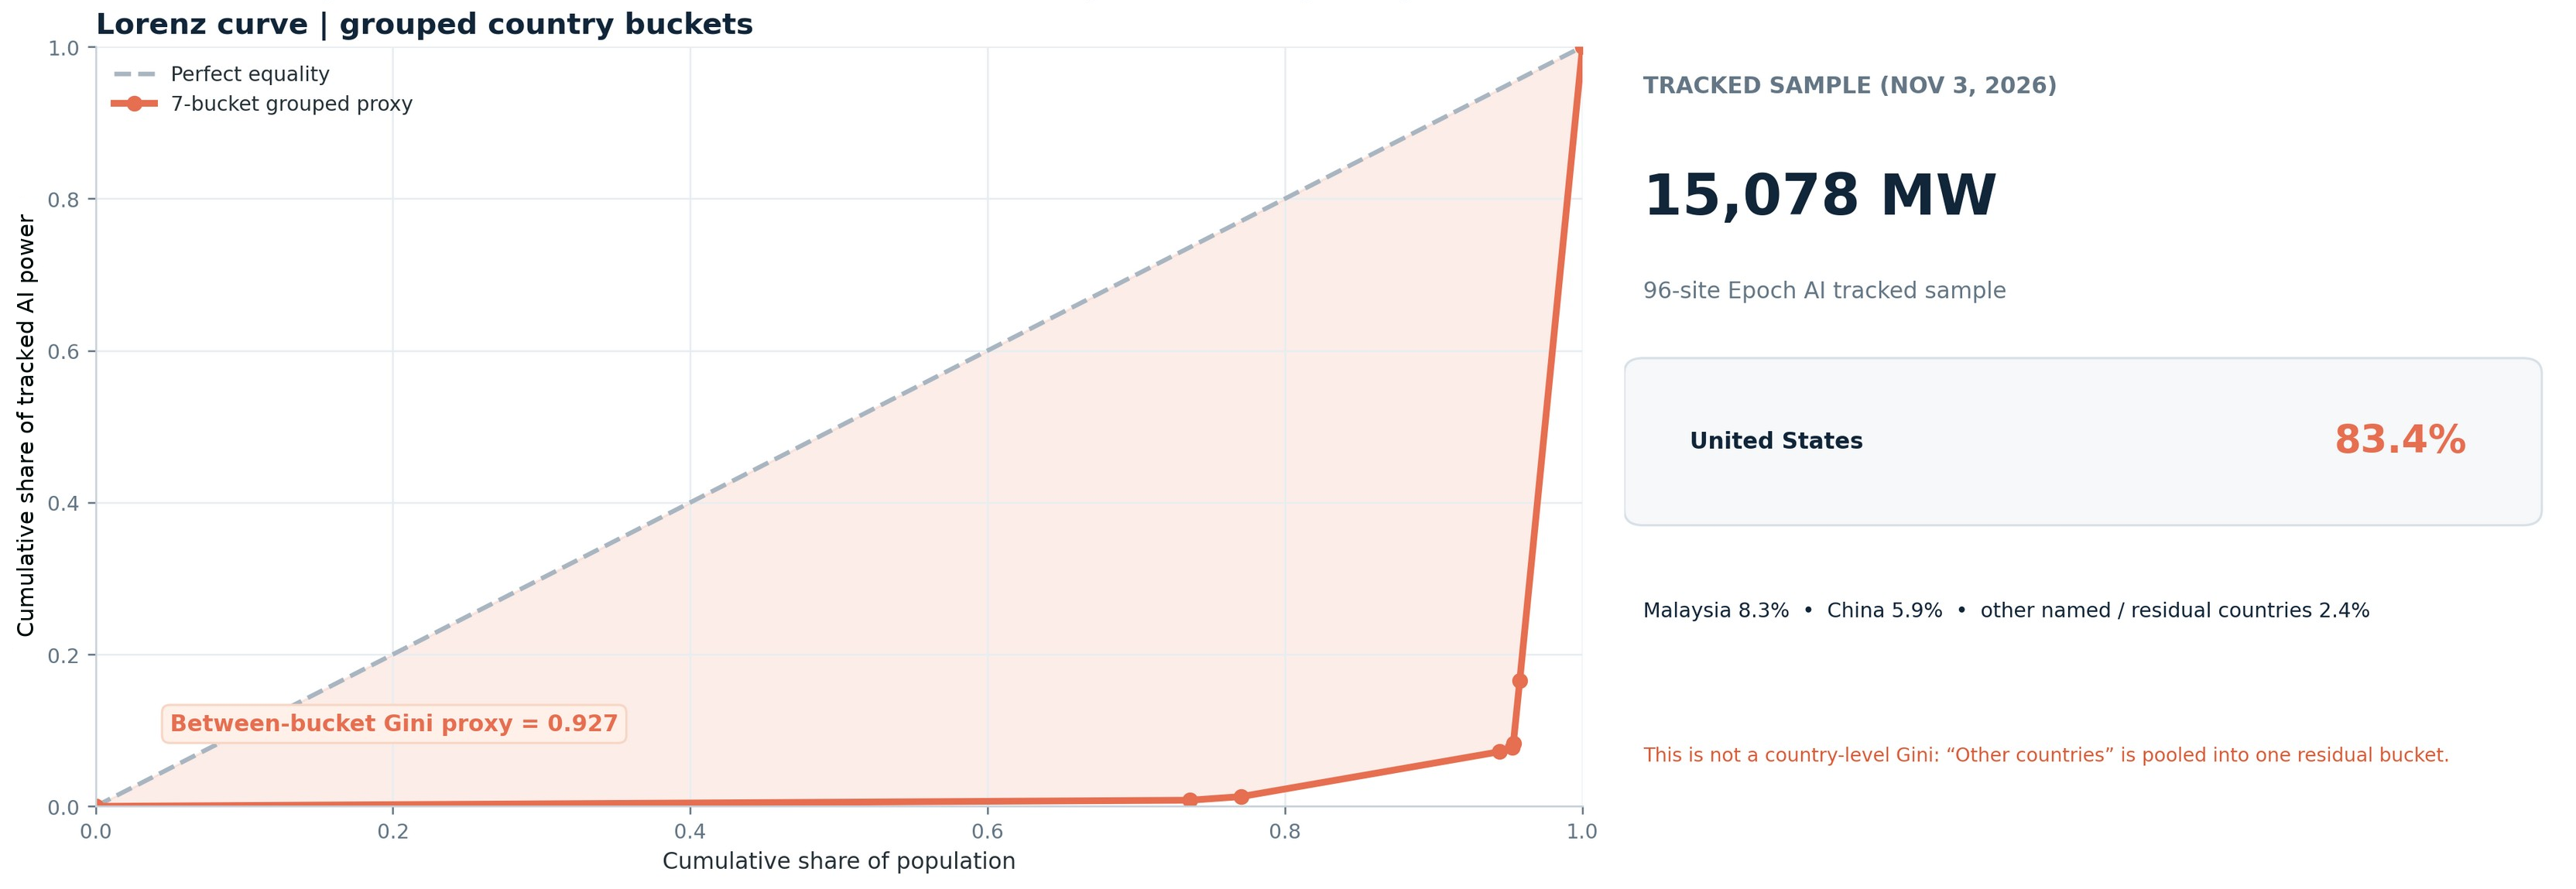
\includegraphics[width=.92\textwidth]{pics/aditya/lorenz_crop.png}\par\smallskip
  \raggedright
  \begin{itemize}\footnotesize
    \item United States 83.4\% of the 15,078 MW tracked; Malaysia 8.3\%; China 5.9\%
    \item Across seven country groups the Gini is \textbf{0.927} (1 = all capacity in one place)
    \item A between-group proxy: pooling ``other countries'' hides inequality within that group
  \end{itemize}
  \src{Epoch AI (2026); UN DESA \emph{World Population Prospects 2024}. Grouping and Gini: project calculation (Aditya).}
  \note{%
    \NoteKey{AI capacity is far more concentrated than people are.}
    \NoteSlide{A Lorenz curve. Horizontal axis: share of the world's population, countries sorted from least to most capacity
    per person. Vertical axis: share of AI capacity. The diagonal is perfect equality; the further the curve sags below
    it, the more unequal. Gini 0.927 (0 = equal, 1 = all in one place). The US holds 83.4\% of 15,078 MW.}
    \NoteWhy{Most of the world hosts almost none of this capacity, so the local costs fall on a few places.}
    \NoteSay{40}{This curve compares where AI capacity is with where people live. If capacity followed population, the curve
    would sit on the diagonal. Instead it hugs the bottom and shoots up at the end: the US alone holds 83\% of what we
    track. Across seven country groups the Gini coefficient is 0.93, close to the maximum.}
    \begin{NoteAsk}
      \item \emph{Why seven groups, not all countries?} A first estimate; pooling ``other countries'' hides inequality inside
        that group. The country-level Gini comes in the report.
    \end{NoteAsk}
  }
\end{frame}

\begin{frame}{Local opposition is rising: \$130 bn of US projects blocked or delayed}
  \centering
  \bignum[phaseAI]{2×}{active opposition groups since\\end-2025, now in 49 US states}\hfill
  \bignum[phaseAI]{75+}{US data-centre projects\\blocked or delayed (Q1 2026)}\hfill
  \bignum[phaseAI]{\$130 bn}{value of the affected\\projects}\par
  \vspace{8pt}
  \raggedright
  {\scriptsize\renewcommand{\arraystretch}{1.15}
  \begin{tabularx}{\textwidth}{@{}>{\bfseries}l X@{}}
    \toprule
    Grievance & What is disputed (tags for coding each case) \\
    \midrule
    Water & Cooling withdrawals, basin stress, competition with households and farms \\
    Power & Grid connection, new generation, electricity bills, fossil lock-in \\
    Noise & Cooling fans, chillers, backup generators \\
    Land & Campus footprint, rezoning, habitat loss, traffic \\
    Jobs & Construction vs permanent jobs; local hiring \\
    \bottomrule
  \end{tabularx}}
  \src{Data Center Watch (2026) \emph{Q1 2026 report}; tags adapted from EJAtlas (Temper et al.\ 2015): a coding framework, not measured totals. Both our cases are about water.}
  \note{%
    \NoteKey{Local resistance is now large enough to block or delay billions of dollars of projects.}
    \NoteSlide{Data Center Watch, US, first quarter of 2026: opposition groups doubled since the end of 2025 and are now in
    49 states; at least 75 projects were blocked or delayed, worth about \$130 billion. The table lists five grievance
    types (water, power, noise, land, jobs) used to code each dispute.}
    \NoteWhy{This is the local scale pushing back. Both our case studies are water disputes.}
    \NoteSay{40}{The local scale is pushing back. In the US, opposition groups doubled in a few months and now exist in 49
    states, and in just the first quarter of 2026 at least 75 projects worth about 130 billion dollars were blocked or
    delayed. The complaints fall into five types: water, power and electricity bills, noise, land, and the jobs promised.}
    \begin{NoteAsk}
      \item \emph{Is there global data?} These figures are US only. The five types follow the EJAtlas categories; a global
        count was not done.
    \end{NoteAsk}
  }
\end{frame}

% ================================================================ O4
\subsection{O4 · Synthesis}

\begin{frame}{Each pressure has its own scale}{}
  {\tiny\renewcommand{\arraystretch}{1.08}
  \begin{tabularx}{\textwidth}{@{}>{\bfseries\raggedright\arraybackslash}p{2.2cm} >{\raggedright\arraybackslash}p{1.45cm} >{\raggedright\arraybackslash}X >{\raggedright\arraybackslash}X >{\raggedright\arraybackslash}X@{}}
    \toprule
    Boundary & Status (2025) & Local & Regional & Global \\
    \midrule
    Climate change & Transgressed & D\enspace Backup generators; construction & \textbf{Q}\enspace Grid intensity 212–559 gCO\textsubscript{2}/kWh & D\enspace Operational and embodied GHG \\
    Freshwater change & Transgressed & \textbf{Q}\enspace 34\% of capacity in stressed basins; Mesa up to 15 M L/day & \textbf{Q}\enspace 67–86\% of water used at power plants & \textbf{Q}\enspace <0.1\% of Earth3's limit: the total hides the hotspots \\
    Land-system change & Transgressed & D\enspace Campus and substation footprint & D\enspace Transmission corridors; mining land & D\enspace Land conversion in the supply chain \\
    Biosphere integrity & Transgressed & D\enspace Habitat effects of sites & D\enspace Mining, river and wetland pressure & D\enspace Cumulative ecosystem pressure \\
    Biogeochemical flows & Transgressed & N & D\enspace Generation, mining and runoff & N \\
    Novel entities & Transgressed & D\enspace Refrigerants, chemicals, exhaust & \textbf{Q}\enspace E-waste collected: 43\% in Europe, 0.7\% in Africa & D\enspace Hazardous material flows \\
    Ocean acidification & Transgressed & N & N & D\enspace Through CO\textsubscript{2} only \\
    Aerosol loading & Safe & D\enspace Diesel and construction particulates & D\enspace Combustion pollution & N \\
    Ozone depletion & Safe & N & N & N \\
    \bottomrule
  \end{tabularx}}
  \par\smallskip
  {\tiny \textbf{Q} quantified in this project\quad D documented pathway, not quantified\quad N not assessed.\quad
  Status is a global assessment, not a finding that data centres caused it.\par}
  \src{Sakschewski et al.\ (2025) \emph{Planetary Health Check}; Richardson et al.\ (2023); Rockström et al.\ (2023); project evidence, slides 17–32}
  \note{%
    \NoteKey{Each pressure lands at its own scale, and that decides who has to respond.}
    \NoteSlide{Rows: the nine planetary boundaries with their 2025 status. Columns: local, regional, global. In each cell,
    Q = we quantified it, D = a documented pathway we did not measure, N = not assessed. The strongest evidence is for
    freshwater (local and regional) and for climate through the grid.}
    \NoteSay{45}{This matrix pulls everything together. Each row is a planetary boundary, each column a scale. Water is
    clearly local and regional: stressed basins, power-plant cooling. Carbon is set regionally by the grid but adds up
    globally. Minerals and e-waste move through global supply chains. We mark honestly what we measured, Q, and what is
    only a documented pathway, D.}
    \begin{NoteAsk}
      \item \emph{Do data centres cause these boundary crossings?} No. The status column is a global assessment of all
        human activity.
    \end{NoteAsk}
  }
\end{frame}
